%\subsubsection{Desenvolvimento}

	%01 - Criação do database
	
	\par Com o ambiente de desenvolvimento pronto, podia-se começar de fato a
desenvolver. Primeiramente foi necessário criar o banco dedados no SGDB. O
banco foi criado, porém sua estrutura não foi definida, pois como será
visto mais adiante o \textit{Hibernate}, possui um mecanismo, que com algumas
configurações, permite a estruturação do banco de dados, de acordo com o
mapeamento objeto relacional. Isto permitirá mudanças na estrutura do banco de
dados e suas tabelas, e até mesmo eventuais correções.

	%02 - Início do projeto web com maven no eclipse;

	\par Em seguida foi criado um projeto do tipo \textit{web} no \textit{Eclipse}
com a ajuda do plugin \textit{Maven}. O \textit{archetype} usado foi
\textit{Quick Star WebApp}. Esse Projeto foi criado usando o \textit{Maven}
pois depende de uma quantidade considerável de \textit{frameworks}, e uma das
principais funcionalidades deste plugin, é ajudar na resolução das dependências
de um projeto Java.

	\par Para tal projeto foi necessário a configuração do \texttt{POM.xml} que é o
arquivo utilizado pelo \textit{Maven}. Nele estão contidas as configurações
relativas à compilação do projeto bem como suas dependências.  Na figura
\ref{fig:desws} a seguir pode ser visto o conteúdo do arquivo
\texttt{POM.xml}.

\begin{figure}[h!]
	\centerline{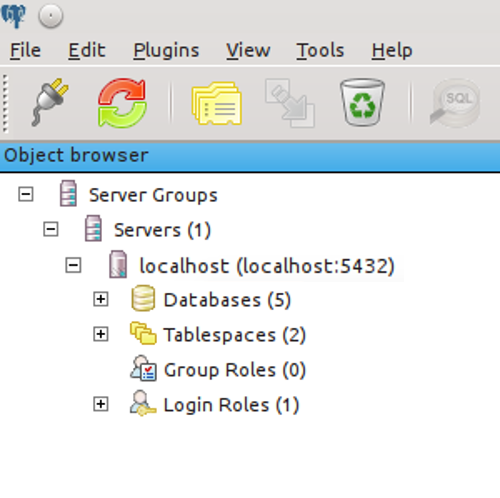
\includegraphics[scale=0.8]{./imagens/2_q_metodologico/4_procedimentos_resultados/43_webservice/432_desenvolvimento/desws.png}}
	\caption[\texttt{pom.xml}]{\texttt{pom.xml}.
		\textbf{Fonte:}Elaborado pelos autores.}
	\label{fig:desws}
\end{figure}

	%03 - Mapeamento orm;
		%	->Criação do pacote

	\par Com a estrutura do projeto devidamente criada foi possível iniciar os
trabalhos com a \\ camada de persistência de dados do projeto. Para este
propósito, primeiramente foi criado um pacote, onde ficaram contidas as classes
que representam as entidades do ORM. O pacote recebeu o nome de
"\texttt{br.edu.univas.restapiappunivas.model}", pois nele estão contidas as
classes que fazem parte do modelo de negócios da aplicação. Este pacote foi
criado visando a divisão das responsabilidades internas no projeto, além de
contribuir positivamente com a organização do mesmo. Tal pacote e as classes
que a estão representandos na figura \ref{fig:desws1}.

\begin{figure}[h!]
	\centerline{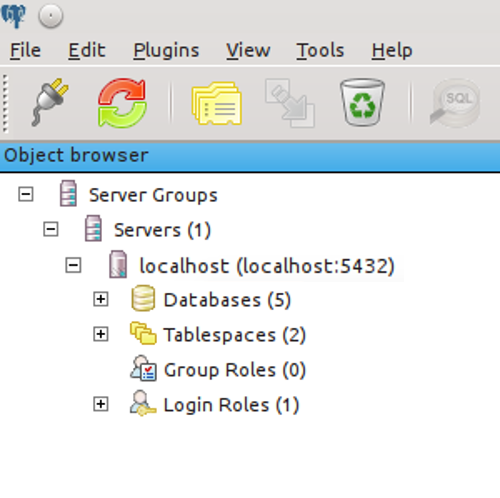
\includegraphics[scale=0.8]{./imagens/2_q_metodologico/4_procedimentos_resultados/43_webservice/432_desenvolvimento/desws.png}}
	\caption[Estrutura do Projeto]{Estrutura do Projeto.
		\textbf{Fonte:}Elaborado pelos autores.}
	\label{fig:desws1}
\end{figure}
		
		%	->Criação das classes
	\par Com este pacote criado, ja era possível criar as classes do ORM. Foi
criada primeiramente a classe \texttt{Student.java}. Para que esta classe
pudesse ser reconhecida como um entidade e persistida ao banco de dados através
do \textit{Hibernate}, é necessário que esta classe tivesse a anotação
\texttt{@Entity}. Esta classe representa a tabela \texttt{students} no banco de
dados.





%04 - HashCode e equals
%05 - Configuração do persistence.xml
%06 - Confecção JpaUtil.java
%07 - Explicar anotações dos pojos
%08 - Finalizando camada de persistência
%09 - Camada de serviço
%10 - Classes que disponibilizam serviços anotações
%11 - Explicar as entities criadas para disponibilizar os dados
%12 - Ctrls que fazem a busca dos dados
%13 - Problema do erro 500
%14 - Provedor de arquivos e contexto
%15 - Em todos citar o pom.xml
%16 - Configuração do web.xml
%17 - Módulo de varredura de atualizações com timerTask
%18 - Módulo de alerta de provas agendas no dia da prova
%19 - Configuração da conta no gcm
%20 - Módulo para disparar as mensagens para o gcm
%21 - Mostrar a estrutura do empacotamento depois de finalizado
%22 - Serviço que faz o registro de sender_id
%23 - Módulo que ira fazer a busca dos dados na base da instituição de ensino
%24 - Falar que vai ser simulado